% Printed 488; principal PDF 495; Google PDF 499.
\par\clearpage
\noindent\makebox[0pt][l]{\fontsize{13}{16}\selectfont 488}\hfill{\small\textbf{POSTHUMOUS PAPERS.}}\hfill\null\par\medskip
\noindent couple of third-rank ones for reconnaissance. I took sole responsibility for all the measurements with the former.

\par\noindent\hspace*{\parindent}In the new undertaking, which concerns the geography of the country more directly and requires a great many secondary and tertiary measurements, several theodolites of the second and third ranks will therefore also be in constant use. Captain \textsc{Müller} used a second-rank theodolite (which the observatory has owned since 1813) last summer, in fact making his first practice observations with it. Lieutenant \textsc{Hartmann} himself owns another (though it is not entirely satisfactory), with which he made his measurements last year. My son used an English third-rank theodolite, which was likewise not particularly good and frequently went out of adjustment. If another second-rank instrument had been available, he could have used it to advantage.

\par\noindent\hspace*{\parindent}I had already ordered a more suitable third-rank theodolite in Munich in the spring of 1828. It arrived in the autumn, cost only a very small sum, and will nevertheless be much more useful for subordinate work and for reconnaissance than the English one mentioned above. Captain \textsc{Müller} acquired a similar one at the same time through my intervention. Reconnaissance work is therefore adequately provided for as long as the staff is not increased.

\par\noindent\hspace*{\parindent}For measurements of the second rank, however, there have so far been far too few instruments available. I therefore ordered another 8-inch theodolite as early as the autumn, and delivery has at least been promised for April of this year.

\par\noindent\hspace*{\parindent}As for the first-rank measurements, which I have taken entirely upon myself so far, I hope it will later be possible to train the other officers gradually in such finer work as well. It will then be most desirable and beneficial to the work if at least two suitable instruments can be used for it. Besides ordering the 8-inch theodolite last autumn, I would therefore have placed an order for a 12-inch one at the same time, had I not already had the prospect of obtaining such a 12-inch theodolite by other means,

% Printed 489; principal PDF 496; Google PDF 500.
\par\clearpage
\noindent\null\hfill{\small\textbf{MEASUREMENT ERRORS.}}\hfill\makebox[0pt][r]{\fontsize{13}{16}\selectfont 489}\par\medskip
\noindent without drawing on the funds for the survey. I knew, namely, that there was a wish to obtain such an instrument for the General Staff Academy. After making several inquiries about this with Mr. \textsc{Ertel} in Munich, I did in fact order such a 12-inch theodolite in Munich at the request of Lieutenant Colonel \textsc{Prott}. It will hopefully be completed in the course of the summer and then be of use in the hands of Captain \textsc{Müller} once he has had the necessary practice.

\par\noindent\hspace*{\parindent}The Munich prices for instruments of this kind are, incidentally, extremely moderate. The 12-inch theodolite, which I have used since 1822 for all the angular measurements in the arc measurement, cost only 800 gulden (light gold). The 8-inch instrument mentioned above (admittedly \textls[120]{somewhat} worn over the 16 years but still very useful) cost 400 gulden at the time. The two of similar dimensions now on order for the General Staff Academy and the trigonometric survey, respectively, will each be considerably less expensive, since I specified a simpler design in several respects (without compromising the \textls[120]{essential point}).

\par\noindent\hspace*{\parindent}In a very large undertaking it is certainly very advantageous to be able to employ a substantial number of theodolites, for quicker progress and proper coordination and thus even with regard to the overall costs. According to a private report, 160 theodolites will be in use in France next summer. Given our small country and the limited staff available for the trigonometric measurements who have already gained some practice, however, I believe we can make do for the present at least with the instruments we have and those now being made. Furthermore, as I had the honour of telling you in person, a trigonometric survey is also planned in the Duchy of Brunswick, for which I have already ordered a 12-inch theodolite. It will probably be possible to arrange these surveys so that they fit together and support one another to their mutual advantage.
\begin{center}\rule{3.5cm}{.4pt}\end{center}
\noindent\makebox[0pt][l]{\small IX.}\makebox[.86\linewidth][r]{62}\par

% Printed 490; principal PDF 497; Google PDF 501.
\par\clearpage
\noindent\makebox[0pt][l]{\fontsize{13}{16}\selectfont 490}\hfill{\small\textbf{CORRESPONDENCE.}}\hfill\null\par\bigskip
\begin{center}{\large [On Measurement Errors.]}\par\bigskip
{\large\textsc{Gauss} to \textsc{Olbers}.\quad Gnarrenburg, July 1825.}\end{center}
\par\noindent\hspace*{\parindent}.\ .\ .\ .\ .\ .\enspace I look back with some dissatisfaction on my 5 years of measurements. As I near the end of them, I find myself in much the same situation and with much the same feelings as many, perhaps most people may have about their life on earth as they approach its end. I feel that there might have been much more satisfaction if I could have begun again with the experience I had gathered, which had come to maturity and clarity only late, with fresh strength and with the appreciation I had acquired of many things. As regards the measurements, I am now convinced of the following.

\par\noindent\hspace*{\parindent}1) A theodolite built like mine gives all angles too small, on average by an amount that is indeed very small but, given the instrument's excellence in other respects, can still be specified very precisely if one observes \textls[120]{only under favourable} conditions. This amount is almost independent of the magnitude of the angles. It almost seems that the \textls[120]{first} turn is chiefly responsible for it, the pivot having been held to some degree, as if by suction. The amount may of course increase as the instrument wears. My measurements at Jever, designed ex professo to determine this amount as well, give $0\overset{\prime\prime}{,}4$, and I do not believe this figure is off by $0\overset{\prime\prime}{,}1$. Unfortunately, my earlier measurements offer no means of determining it so conclusively. Although I suspected the existence of this source of error from the very beginning, I thought it too small to be treated otherwise than as $=0$. Had I been conducting a survey of the country instead of an arc measurement and thus had more frequent opportunity for a Gyrus horizontis, I would undoubtedly have given up this view sooner. Next winter I shall try to determine the amount for each year as well as I can. I am now convinced that if, first, this amount is always taken into account, if, second, all measuring is suspended when the circumstances are unfavourable, and if, third, the other two circumstances still to be mentioned are heeded, then measurements on heliotrope light can attain an almost incredible precision from which I

% Printed 491; principal PDF 498; Google PDF 502.
\par\clearpage
\noindent\null\hfill{\small\textbf{MEASUREMENT ERRORS.}}\hfill\makebox[0pt][r]{\fontsize{13}{16}\selectfont 491}\par\medskip
\noindent now unfortunately remain much further removed. An analysis of the measurements made in Göttingen in 1823 gives me the above amount $=0\overset{\prime\prime}{,}140$, though only with a weight of 47 repetitions. Even then the probable error is only almost exactly $\pm0\overset{\prime\prime}{,}140$, so that one can wager 1 to 1 that the amount lies within the limits $0$ and $+0\overset{\prime\prime}{,}28$. The measurements on the Timpenberg in 1823 gave the amount $+0\overset{\prime\prime}{,}070$ with weight 28. If they may be combined, the value for 1823 would be
\[
+0\overset{\prime\prime}{,}114\ \text{with weight }75.
\]
\par\noindent\hspace*{\parindent}I shall work through all the stations in turn and then take the effect into account in the calculation.

\par\noindent\hspace*{\parindent}2) One should observe only under favourable conditions, when the air does not shimmer, no wind shakes the instrument, and the mounting is quite solid. Admittedly there will then often be weeks in which one cannot observe at all, and rarely will one observe for more than 1--2 hours on any one day, high mountain stations perhaps excepted. On the other hand, 50 such measurements are worth more than 500 made under unfavourable conditions. \textls[120]{Our} instruments, if their excellence is \textls[120]{fully} put to use, are actually too good for the usual state of the atmosphere. The errors from shimmer in the air are ten times as great as the unavoidable ones due to the instrument. The same probably applies to astronomical observations.

\par\noindent\hspace*{\parindent}3) Whenever possible, the heliotrope lights should appear completely unobstructed. Where that is impossible, one should sight \textls[120]{never between the threads}, but always on one of them. Otherwise the bias of the bisection can produce an error that acts in the same direction and may rise to $1\frac12$ to $2''$. I have always suspected that such an error could arise, but without the experience at Langwarden I would never have believed it was so large. I often sighted \textls[120]{on} the thread in the past, though almost only where the light appeared unobstructed, and in that case I never found a marked difference. I therefore abandoned that way of observing --- which I \textls[120]{now} regret --- because it was much more troublesome for me, and I believed, certainly with good reason in \textls[120]{general}, that I could not sight as precisely on the threads as between them.

\par\noindent\hspace*{\parindent}4) Even so, I am convinced that instances of lateral refraction
\par\medskip\noindent\makebox[.86\linewidth][r]{62\textsuperscript{*}}\par

% Printed 492; principal PDF 499; Google PDF 503.
\par\clearpage
\noindent\makebox[0pt][l]{\fontsize{13}{16}\selectfont 492}\hfill{\small\textbf{CORRESPONDENCE.}}\hfill\null\par\medskip
\noindent do occur, acting in a constant direction at the time of day suitable for observing, when the light passes close by trees, etc. The circumstances listed above under 1) to 3) are not strong enough in several triangles to explain the large anomalies in the sum of the angles. In the triangle Garlste-Lehe-Varel, for example, where the sum of the errors is $4\overset{\prime\prime}{,}9$, they could hardly account for more than $1\frac12$ to $2''$, and the remainder is still much too large to be ascribed to irregular measurement errors. Much to my displeasure, such a lateral refraction certainly also occurs on the side Brillit-Lehe, with the effect that here too the angles come out too small. The very costly cut through the trees originally went too far to the left. It was widened a little more so that Lehe became visible here, but so close to the right-hand wall that there is certainly lateral refraction. I shall try to have some projecting branches with dense foliage located and removed. It is uncertain, however, whether they will be found, and even then the line of sight will still pass very close to the right-hand wall. Unfortunately the angle at Lehe has in any event very probably been strongly affected by this already, and I would be reluctant to go back there unless it were possible to make Bremervörde, which is said to be visible at Lehe, visible at Brillit and at Zeven. Unfortunately, besides fruit trees, a farmhouse also appears to stand in the direction Brillit-Bremervörde, though I do not yet know this for certain, since I still have no means of specifying the azimuth with any confidence. Otherwise I am sure this new connection would shed a great deal of new light. The angle at Brillit between Zeven and Bremen seems likely to improve by $2''$, i.e. to increase, bringing the sum of the errors from $4\frac12{}''$ down to
\begin{center}
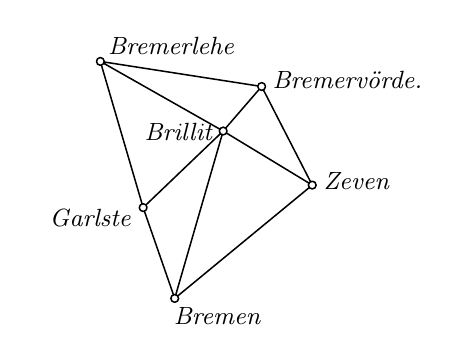
\begin{tikzpicture}[x=.0055cm,y=-.0055cm,line width=.55pt,line cap=round,line join=round,
 every node/.style={font=\small\itshape,inner sep=1pt}]
\path[use as bounding box] (0,0) rectangle (930,700);
\coordinate (Lehe) at (168,78); \coordinate (Voerde) at (541,136);
\coordinate (Brillit) at (452,239); \coordinate (Zeven) at (658,364);
\coordinate (Garlste) at (267,416); \coordinate (Bremen) at (340,626);
\draw (Lehe)--(Voerde)--(Zeven)--(Bremen)--(Garlste)--(Lehe)
 (Lehe)--(Brillit)--(Zeven) (Voerde)--(Brillit)--(Garlste) (Brillit)--(Bremen);
\foreach \v in {Lehe,Voerde,Brillit,Zeven,Garlste,Bremen}
 \draw[fill=white] (\v) circle[radius=1.4pt];
\node[anchor=south west] at (178,70) {Bremerlehe};
\node[anchor=south west] at (558,148) {Bremervörde.};
\node[anchor=east] at (434,240) {Brillit};
\node[anchor=west] at (676,354) {Zeven};
\node[anchor=east] at (246,439) {Garlste};
\node[anchor=north west] at (330,638) {Bremen};
\end{tikzpicture}
\end{center}
\noindent $2\frac12{}''$. But this remainder, too, certainly cannot be ascribed entirely to measure-

% Printed 493; principal PDF 500; Google PDF 504.
\par\clearpage
\noindent\null\hfill{\small\textbf{MEASUREMENT ERRORS.}}\hfill\makebox[0pt][r]{\fontsize{13}{16}\selectfont 493}\par\medskip
\noindent ment errors. In Bremen in particular, error 1) above is almost completely eliminated by measuring forwards and backwards, and the manner of sighting can also have little effect, since, given the considerable distance and the usual invisibility of the towers, the lights appeared virtually unobstructed.\par
\noindent .\ .\ .\ .\ .\ .
\begin{center}{\large\textsc{Gauss} to \textsc{Schumacher}.\quad Göttingen, 14 August 1825.}\end{center}
\par\noindent\hspace*{\parindent}.\ .\ .\ .\ .\ .\enspace Significant anomalies in my measurements have caused me great trouble this summer. I am now convinced that strong lateral refractions can occur in flat country when the light passes very close over or beside woodland and that in the hours suitable for measuring they always act in one direction. But it is just as certain that they have combined with other sources of error that I have now fairly well traced. The following two in particular.\quad 1) Sighting heliotrope light \textls[120]{between} the threads, especially when the light is faint, is unsuitable if it is not unobstructed but is, for example, off centre in the lantern of a tower that is itself fairly clearly visible. Constant errors of more than $2''$ can thus arise. Since becoming convinced of this, I have always sighted \textls[120]{on} one thread in such cases and have thereby obtained a considerable reduction in some of the anomalies.\quad 2) Theodolites built like ours decidedly give all angles too small, and the mean value of the error (which seems to depend little on the magnitude of the angle) can be determined very precisely, but may keep increasing as the instrument wears. At Brillit I found $0\overset{\prime\prime}{,}723$, with a probable error that will be under $0\overset{\prime\prime}{,}1$. At Jever I had only about $0\overset{\prime\prime}{,}5$. I am not yet sure whether the main source of the error lies in the graduated-circle clamp (particularly the ball), in the sleeve that carries the lower telescope, or in the screw that holds the sleeve against the base of the instrument. The last of these is fairly worn on my instrument, and to make some trials I am now having the graduated-circle clamp attached directly to the base of the instrument, in which case I shall remove the lower telescope altogether. I consider it not only useless where one has a solid mounting but detrimental, inasmuch as its sleeve, which serves as an intermediate part in fastening the

% Printed 494; principal PDF 501; Google PDF 505.
\par\clearpage
\noindent\makebox[0pt][l]{\fontsize{13}{16}\selectfont 494}\hfill{\small\textbf{CORRESPONDENCE.}}\hfill\null\par\medskip
\noindent graduated circle to the base, multiplies the risk of the graduated circle moving when it is assumed to be fixed. I would have liked very much to speak to you at some length about these matters and to exchange my experiences and views with yours.
\par\bigskip
\begin{center}{\large\textsc{Gauss} to \textsc{Bessel}.\quad Göttingen, 29 October 1843.}\end{center}
\par\noindent\hspace*{\parindent}.\ .\ .\ .\ .\ .\enspace This concerns a finding that has often troubled me, namely that theodolites built to \textsc{Reichenbach}'s design tend to give all angles too small. Perhaps you have had similar experiences, which I would gladly compare with my own.

\par\noindent\hspace*{\parindent}For my angular measurements in the arc measurement from 1821 to 1823 and for the subsequent extension of my triangles in 1824 and 1825, I used two different 12-inch theodolites (verniers reading to $4''$, magnification about 35 times). The one, which \textsc{Schumacher} lent me, was made by \textsc{Reichenbach} himself and I used it only in 1821. The other, made by \textsc{Ertel}, was exactly like it and belongs to the observatory. I used it from 1822 to 1825. I did not notice the phenomenon at all with the first instrument, or with the second in the first three years or in early 1825. It was only in the latter half of the measurements that I noticed it, on a small scale, to be sure, but so distinctly that there could be no doubt about it. An explanation, at least of the principal source, is indeed close at hand. For brevity I call the two objects $A$, $B$ and assume that $B$ lies to the right of $A$ and that the first sighting is always at $A$ and the second at $B$. After taking a reading and setting the instrument on $A$, one unclamps the alidade and moves it to reach $B$. The assumption that the circle itself remains \textls[120]{absolutely} fixed during this motion is precarious, however. If there is the slightest play, imperceptible in itself, the turning of the alidade will carry the circle round a little in the same direction (from left to right). The difference of the readings will therefore give too small an angle. No matter how many repetitions there are, the final result will always remain too small.

\par\noindent\hspace*{\parindent}Once I had recognised this, I adopted the expedient (at Jever) of always adding to a number of repetitions made in the usual way

% Printed 495; principal PDF 502; Google PDF 506.
\par\clearpage
\noindent\null\hfill{\small\textbf{MEASUREMENT ERRORS.}}\hfill\makebox[0pt][r]{\fontsize{13}{16}\selectfont 495}\par\medskip
\noindent an equal number in which I\ \raisebox{1.5ex}{\scriptsize.}\ moved the alidade from right to left through the supplement to $360^\circ$. All the angles now invariably came out larger than before, and the difference, averaging about 2 arcseconds, seemed to depend either not at all, or at least not perceptibly, on the magnitude of the angles. The mean of the two results could therefore be taken as the true value of the angle, and indeed all the results obtained in this manner, at this station as well as at the others, were entirely satisfactory. Thus the theodolite in its condition at that time appeared to give all angles measured in the usual way about one arcsecond too small.

\par\noindent\hspace*{\parindent}The motion of the entire circle from the first reading to the first\linebreak
sighting, and subsequently from the \begin{tabular}[c]{@{}c@{}}2.\\4.\\6.\end{tabular}\ etc. to the \begin{tabular}[c]{@{}c@{}}3.\\5.\\7.\end{tabular}\ etc. sighting, was always from\linebreak
right to left (through the angle $<180^\circ$). It is at least conceivable that an effect in a constant direction may occur here too. If part of the play is in the adjusting screws, nuts or balls, a slight shift of the reading may also occur while the whole circle is turning, owing to the friction of the alidade pivot on the springs supporting it from below. This would have exactly the opposite effect and would thus help to increase the angles. I assumed, however, that this effect was imperceptible. It would take a very great deal of time to settle the matter a posteriori. I need hardly mention that I \textls[120]{always} made sure the adjusting screws did not turn too freely.

\par\noindent\hspace*{\parindent}It must undoubtedly be due to play somewhere, but it is hard to ascertain \textls[120]{where} chiefly. I subsequently had this theodolite modified to remove any play that could conceivably occur in the turning motion by which the check telescope is moved. I discarded the check telescope altogether, as it is wholly useless with a firm mounting, and had the arm bearing the circle clamp fastened directly to the base with strong angle brackets. However, too few measurements have been made with the instrument \textls[120]{after} this change for its effect to be judged with certainty.

% Printed 496; principal PDF 503; Google PDF 507.
\par\clearpage
\noindent\makebox[0pt][l]{\fontsize{13}{16}\selectfont 496}\hfill{\small\textbf{CORRESPONDENCE.}}\hfill\null\par\medskip
\par\noindent\hspace*{\parindent}For the later measurements from 1828 to 1843 my officers used three other theodolites.
\par\noindent\hspace*{\parindent}1) \textsc{Hartmann} used an 8-inch \textsc{Reichenbach} theodolite, which the observatory had owned since 1813.
\par\noindent\hspace*{\parindent}2) \textsc{Müller} used a 12-inch \textsc{Ertel} theodolite belonging to the Hanoverian General Staff (I procured it), very similar to the one above but without a vertical circle or a check telescope.
\par\noindent\hspace*{\parindent}3) My son used an 8-inch \textsc{Ertel} theodolite, also without a vertical circle or a check telescope but with a telescope of exactly the same power as No. 2. The vernier in this one reads to $10''$.

\par\noindent\hspace*{\parindent}The phenomenon did not become apparent in No. 1. The instrument was used for only a couple of years, and the results for the angles were always very good indeed. The telescope has weaker optical power, but \textsc{Hartmann} always fitted another, more powerful telescope of his own. I mention this circumstance only to explain why \textls[120]{this} theodolite was no longer used afterwards.

\par\noindent\hspace*{\parindent}I am writing about No. 2 from memory alone and cannot say exactly at this moment \textls[120]{when} the phenomenon began to appear. If I am not mistaken, there was no particular trace of it in the first years, but in later years it was unmistakable and at least twice as large as in the instrument I used. That theodolite was often taken apart and cleaned and, if I recall correctly, was also fitted with new adjusting screws by \textsc{Hohnbaum} in Hanover, without eliminating the error. I always strongly recommended the above-mentioned remedy to the late \textsc{Müller}, but I do not think he always applied it consistently.

\par\noindent\hspace*{\parindent}With No. 3 my son made \textls[120]{very} extensive measurements in the years 1829, 1830, 1831, 1833. The angles (incidentally, \textls[120]{all} combinations between all principal directions are generally measured at every station, as you can also see from \textsc{Gerling}'s work) always agreed to my complete satisfaction, at least as well as or almost better than \textsc{Müller}'s with No. 2, and the error at any rate did not appear to any appreciable degree.

\par\noindent\hspace*{\parindent}From 1834 this theodolite was used for about 5 or 6 years at the magnetic observatory, and later at times by \textsc{Goldschmidt} for angular measure-

% Printed 497; principal PDF 504; Google PDF 508.
\par\clearpage
\noindent\null\hfill{\small\textbf{MEASUREMENT ERRORS.}}\hfill\makebox[0pt][r]{\fontsize{13}{16}\selectfont 497}\par\medskip
\noindent ments, but these were of too minor a nature for the above error to have come into question.

\par\noindent\hspace*{\parindent}My son used this same theodolite No. 3 again last summer for principal angles. At the stations where most of the angles were measured (towers in Hamburg and Stade), the circumstances were extremely unfavourable in many respects. Nevertheless, the presence of that negative error, now probably amounting to 3 to $4''$, was quite unmistakable. The theodolite had been cleaned and inspected here before being sent out, and no play whatever had been noticed. My son found, however, that the end of the circle's adjusting screw was fairly worn, so the observations of the first days, when this had gone unnoticed, were discarded. Later the use of this part of the screw was carefully avoided, and no play could be detected in it. I shall now have the theodolite brought back here and try to see whether modifications can remedy the error or at least its effect. I shall have new clamp jaws made. I have yet to decide whether to have entirely new screws made with their fittings, for fear of going from bad to worse. Since you yourself have received a small theodolite from \textsc{Meyerstein}, I ask you to examine precisely \textls[120]{this} part of the work with great care and tell me your findings in confidence. I also have an idea for a remedy that will admittedly leave the error (a hidden looseness) in place but may, I hope, render it harmless.

\par\noindent\hspace*{\parindent}As you know, the pivot of the alidade and the bushing for that pivot, which is itself the pivot of the graduated circle, are each supported from below on separate springs. I intend to have these springs modified so that their tension can be increased or decreased easily and instantly at will. During the measurements the tensions are then to be alternated systematically, so that when the alidade is turned, the springs supporting its pivot are under strong tension and the springs supporting the bushing are under almost none, and the reverse when the whole circle is turned. \textsc{Meyerstein} thinks that he can arrange such a change quite suitably, and I expect a great deal from it. The only pity is
\par\medskip\noindent\makebox[0pt][l]{\small IX.}\makebox[.86\linewidth][r]{63}\par
